% Options for packages loaded elsewhere
\PassOptionsToPackage{unicode}{hyperref}
\PassOptionsToPackage{hyphens}{url}
\documentclass[
  english,
  11pt,
]{article}
\usepackage{xcolor}
\usepackage[a4paper,margin=24mm]{geometry}
\usepackage{amsmath,amssymb}
\setcounter{secnumdepth}{5}
\usepackage{iftex}
\ifPDFTeX
  \usepackage[T1]{fontenc}
  \usepackage[utf8]{inputenc}
  \usepackage{textcomp} % provide euro and other symbols
\else % if luatex or xetex
  \usepackage{unicode-math} % this also loads fontspec
  \defaultfontfeatures{Scale=MatchLowercase}
  \defaultfontfeatures[\rmfamily]{Ligatures=TeX,Scale=1}
\fi
% \usepackage{lmodern}
\ifPDFTeX\else
  % xetex/luatex font selection
\fi
% Use upquote if available, for straight quotes in verbatim environments
\IfFileExists{upquote.sty}{\usepackage{upquote}}{}
\IfFileExists{microtype.sty}{% use microtype if available
  \usepackage[]{microtype}
  \UseMicrotypeSet[protrusion]{basicmath} % disable protrusion for tt fonts
}{}
\makeatletter
\@ifundefined{KOMAClassName}{% if non-KOMA class
  \IfFileExists{parskip.sty}{%
    \usepackage{parskip}
  }{% else
    \setlength{\parindent}{0pt}
    \setlength{\parskip}{6pt plus 2pt minus 1pt}}
}{% if KOMA class
  \KOMAoptions{parskip=half}}
\makeatother
\usepackage{color}
\usepackage{fancyvrb}
\newcommand{\VerbBar}{|}
\newcommand{\VERB}{\Verb[commandchars=\\\{\}]}
\DefineVerbatimEnvironment{Highlighting}{Verbatim}{commandchars=\\\{\}}
% Add ',fontsize=\small' for more characters per line
\newenvironment{Shaded}{}{}
\newcommand{\AlertTok}[1]{\textcolor[rgb]{1.00,0.00,0.00}{\textbf{#1}}}
\newcommand{\AnnotationTok}[1]{\textcolor[rgb]{0.38,0.63,0.69}{\textbf{\textit{#1}}}}
\newcommand{\AttributeTok}[1]{\textcolor[rgb]{0.49,0.56,0.16}{#1}}
\newcommand{\BaseNTok}[1]{\textcolor[rgb]{0.25,0.63,0.44}{#1}}
\newcommand{\BuiltInTok}[1]{\textcolor[rgb]{0.00,0.50,0.00}{#1}}
\newcommand{\CharTok}[1]{\textcolor[rgb]{0.25,0.44,0.63}{#1}}
\newcommand{\CommentTok}[1]{\textcolor[rgb]{0.38,0.63,0.69}{\textit{#1}}}
\newcommand{\CommentVarTok}[1]{\textcolor[rgb]{0.38,0.63,0.69}{\textbf{\textit{#1}}}}
\newcommand{\ConstantTok}[1]{\textcolor[rgb]{0.53,0.00,0.00}{#1}}
\newcommand{\ControlFlowTok}[1]{\textcolor[rgb]{0.00,0.44,0.13}{\textbf{#1}}}
\newcommand{\DataTypeTok}[1]{\textcolor[rgb]{0.56,0.13,0.00}{#1}}
\newcommand{\DecValTok}[1]{\textcolor[rgb]{0.25,0.63,0.44}{#1}}
\newcommand{\DocumentationTok}[1]{\textcolor[rgb]{0.73,0.13,0.13}{\textit{#1}}}
\newcommand{\ErrorTok}[1]{\textcolor[rgb]{1.00,0.00,0.00}{\textbf{#1}}}
\newcommand{\ExtensionTok}[1]{#1}
\newcommand{\FloatTok}[1]{\textcolor[rgb]{0.25,0.63,0.44}{#1}}
\newcommand{\FunctionTok}[1]{\textcolor[rgb]{0.02,0.16,0.49}{#1}}
\newcommand{\ImportTok}[1]{\textcolor[rgb]{0.00,0.50,0.00}{\textbf{#1}}}
\newcommand{\InformationTok}[1]{\textcolor[rgb]{0.38,0.63,0.69}{\textbf{\textit{#1}}}}
\newcommand{\KeywordTok}[1]{\textcolor[rgb]{0.00,0.44,0.13}{\textbf{#1}}}
\newcommand{\NormalTok}[1]{#1}
\newcommand{\OperatorTok}[1]{\textcolor[rgb]{0.40,0.40,0.40}{#1}}
\newcommand{\OtherTok}[1]{\textcolor[rgb]{0.00,0.44,0.13}{#1}}
\newcommand{\PreprocessorTok}[1]{\textcolor[rgb]{0.74,0.48,0.00}{#1}}
\newcommand{\RegionMarkerTok}[1]{#1}
\newcommand{\SpecialCharTok}[1]{\textcolor[rgb]{0.25,0.44,0.63}{#1}}
\newcommand{\SpecialStringTok}[1]{\textcolor[rgb]{0.73,0.40,0.53}{#1}}
\newcommand{\StringTok}[1]{\textcolor[rgb]{0.25,0.44,0.63}{#1}}
\newcommand{\VariableTok}[1]{\textcolor[rgb]{0.10,0.09,0.49}{#1}}
\newcommand{\VerbatimStringTok}[1]{\textcolor[rgb]{0.25,0.44,0.63}{#1}}
\newcommand{\WarningTok}[1]{\textcolor[rgb]{0.38,0.63,0.69}{\textbf{\textit{#1}}}}
\usepackage{longtable,booktabs,array}
\usepackage{caption}
\captionsetup[table]{skip=6pt}
\newcounter{none} % for unnumbered tables
\usepackage{calc} % for calculating minipage widths
% Correct order of tables after \paragraph or \subparagraph
\usepackage{etoolbox}
\makeatletter
\patchcmd\longtable{\par}{\if@noskipsec\mbox{}\fi\par}{}{}
\makeatother
\usepackage{graphicx}
\makeatletter
\newsavebox\pandoc@box
\newcommand*\pandocbounded[1]{% scales image to fit in text height/width
  \sbox\pandoc@box{#1}%
  \Gscale@div\@tempa{\textheight}{\dimexpr\ht\pandoc@box+\dp\pandoc@box\relax}%
  \Gscale@div\@tempb{\linewidth}{\wd\pandoc@box}%
  \ifdim\@tempb\p@<\@tempa\p@\let\@tempa\@tempb\fi% select the smaller of both
  \ifdim\@tempa\p@<\p@\scalebox{\@tempa}{\usebox\pandoc@box}%
  \else\usebox{\pandoc@box}%
  \fi%
}
% Set default figure placement to htbp
\def\fps@figure{htbp}
\makeatother
\ifLuaTeX
\usepackage[bidi=basic,shorthands=off]{babel}
\else
\usepackage[bidi=default,shorthands=off]{babel}
\fi
\ifLuaTeX
  \usepackage{selnolig} % disable illegal ligatures
\fi
\setlength{\emergencystretch}{3em} % prevent overfull lines
\providecommand{\tightlist}{%
  \setlength{\itemsep}{0pt}\setlength{\parskip}{0pt}}
\usepackage[]{natbib}
\bibliographystyle{plainnat}
\makeatletter
\@ifpackageloaded{subcaption}{}{\usepackage{subcaption}}
\@ifpackageloaded{caption}{}{\usepackage{caption}}
\captionsetup[subfigure]{margin=0.5em}
\AtBeginDocument{%
\renewcommand*\figurename{Figure}
\renewcommand*\tablename{Table}
}
\AtBeginDocument{%
\renewcommand*\listfigurename{List of Figures}
\renewcommand*\listtablename{List of Tables}
}
\newcounter{pandoccrossref@subfigures@footnote@counter}
\newenvironment{pandoccrossrefsubfigures}{%
\setcounter{pandoccrossref@subfigures@footnote@counter}{0}
\begin{figure}\centering%
\gdef\global@pandoccrossref@subfigures@footnotes{}%
\DeclareRobustCommand{\footnote}[1]{\footnotemark%
\stepcounter{pandoccrossref@subfigures@footnote@counter}%
\ifx\global@pandoccrossref@subfigures@footnotes\empty%
\gdef\global@pandoccrossref@subfigures@footnotes{{##1}}%
\else%
\g@addto@macro\global@pandoccrossref@subfigures@footnotes{, {##1}}%
\fi}}%
{\end{figure}%
\addtocounter{footnote}{-\value{pandoccrossref@subfigures@footnote@counter}}
\@for\f:=\global@pandoccrossref@subfigures@footnotes\do{\stepcounter{footnote}\footnotetext{\f}}%
\gdef\global@pandoccrossref@subfigures@footnotes{}}
\@ifpackageloaded{float}{}{\usepackage{float}}
\floatstyle{ruled}
\@ifundefined{c@chapter}{\newfloat{codelisting}{h}{lop}}{\newfloat{codelisting}{h}{lop}[chapter]}
\floatname{codelisting}{Listing}
\newcommand*\listoflistings{\listof{codelisting}{List of Listings}}
\makeatother
\usepackage{bookmark}
\IfFileExists{xurl.sty}{\usepackage{xurl}}{} % add URL line breaks if available
\urlstyle{same}
% fallback for those not using the hyperref driver hyperxmp:
\makeatletter
\@ifundefined{xmpquote}{\newcommand{\xmpquote}[1]{#1}}{}
\makeatother
\hypersetup{
  pdftitle={antropy: native multidimensional entropy and configurable complexity analysis},
  pdfauthor={Daniel Ari Friedman},
  pdflang={en},
  colorlinks=true,linkcolor=red,urlcolor=red,citecolor=red,anchorcolor=red,filecolor=red,
  pdfcreator={LaTeX via pandoc}}

\ifXeTeX
\special{pdf:trailerid [ <ad01997d0d0e52c44779c936d64975eb> <ad01997d0d0e52c44779c936d64975eb> ]}
\fi
\ifPDFTeX
\pdftrailerid{}
\pdftrailer{/ID [ <ad01997d0d0e52c44779c936d64975eb> <ad01997d0d0e52c44779c936d64975eb> ]}
\fi
\ifLuaTeX
\pdfvariable trailerid {[ <ad01997d0d0e52c44779c936d64975eb> <ad01997d0d0e52c44779c936d64975eb> ]}
\fi

\title{antropy: native multidimensional entropy and configurable
complexity analysis}
\author{Daniel Ari Friedman}
\date{}

\IfFileExists{seqsplit.sty}{\usepackage{seqsplit}}{\newcommand{\seqsplit}[1]{#1}}
\protected\def\breakseq#1{\seqsplit{#1}}
\protected\def\breaktt#1{\begingroup\ttfamily\seqsplit{#1}\endgroup}
\title{antropy: native multidimensional entropy and configurable complexity analysis}
\author{Daniel Ari Friedman\\\footnotesize{Active Inference Institute}\\\footnotesize{\texttt{daniel@activeinference.institute}}}
\date{}

\usepackage{amsmath}
\usepackage{amssymb}
\usepackage{amsfonts}
\usepackage{amsthm}
\usepackage{booktabs}
\usepackage{longtable}
\usepackage{array}
\usepackage{graphicx}
\usepackage{float}
\usepackage[section]{placeins}
\floatplacement{figure}{p}
\usepackage{listings}
\usepackage{microtype}
\usepackage{xcolor}
\usepackage{fontspec}
\setmonofont{lmmono10-regular.otf}
\newtheorem{theorem}{Theorem}[section]
\newtheorem{remark}[theorem]{Remark}
\newtheorem{example}[theorem]{Example}
\newtheorem{definition}[theorem]{Definition}
\setcounter{tocdepth}{2}
\setcounter{secnumdepth}{3}
\hypersetup{colorlinks=true,linkcolor=blue,citecolor=blue,urlcolor=blue}
\renewcommand{\bibsection}{}

\begin{document}
\begin{titlepage}
\centering
\vspace*{2cm}
{\LARGE\bfseries antropy: native multidimensional entropy and configurable complexity analysis\par}
\vspace{0.75em}
{\large Methods, replicated synthetic studies, and resource-aware reproducibility\par}
\vfill
\makeatletter
{\@author\par}
\vspace{1em}
{\@date\par}
\makeatother
\vfill
\end{titlepage}
\thispagestyle{empty}
\tableofcontents
\newpage

\section*{Abstract}\label{abstract}
\addcontentsline{toc}{section}{Abstract}

antropy: native multidimensional entropy and configurable complexity
analysis provides a configurable framework for native spatial entropy,
probability information, ordinal patterns, spectral distributions and
trajectory structure. The implementation separates local spatial
extraction from pair selection and estimator semantics. A common typed
result preserves finite, undefined and infinite outcomes instead of
collapsing them into missing numeric values. This manuscript accompanies
antropy-hd 0.2.0.

The retained baseline contains 54 measured rows. The configured
replicated study contains 150 fields and 1650 scalar estimates,
including native HDSE, row-major flattened sample entropy and a
fixed-alphabet entropy-complexity plane. Its field sizes are 48, 10 x
12, 6 x 7 x 8, with 5 independent generated trials per condition.
Analytical work estimates report actual blocked-kernel schedules;
empirical runtimes retain their host and repetition metadata. Source
variables, figures and tables are generated from the stored reports and
validated configuration.

The published HDSE construction motivates the local-template estimator,
while the manuscript distinguishes source conventions, ambiguities and
explicit extensions. The experiments are controlled synthetic
demonstrations rather than a reproduction of the source paper's
empirical classification results. Rendering uses the pinned shared
research template's Pandoc, LaTeX, bibliography and real
table-of-contents pipeline.

\section{Introduction}\label{sec:introduction}

Entropy is a family of questions about a specified representation,
population and uncertainty model. A probability entropy asks about
masses over an alphabet. A sample-template estimator asks how frequently
similar local configurations remain similar after their representation
is extended. Ordinal and spectral estimators construct different
distributions. Their outputs require the input meaning, units,
normalization and finite-sample convention to remain visible.

Native multidimensional data make these distinctions especially
consequential. A spatial field has coordinate adjacency along several
axes. Globally flattening it changes which values become adjacent in a
one-dimensional embedding. Native HDSE extracts rectangular local blocks
before their values are arranged for distance computation
\citep{xia2026hdse}. The mathematical estimator and the file
representation are therefore distinct layers.

The repository name combines entropy and ant, reflecting interest in
collective biological organization. No biological observations are
included in the present study. The distribution and Python import use
the separate names \texttt{antropy-hd} and \texttt{antropy\_hd} to
preserve compatibility with the unrelated AntroPy time-series library.
The current registry exposes 19 orchestratable entries, while the
numerical API also exposes reusable geometry, information and
cost-estimation components.

The project has four connected aims: state estimator contracts
precisely; preserve native geometry and explicit degeneracy; produce a
replicated synthetic study with complete result coverage; and bind
measured outputs to executable, resource-aware software and a
configurable manuscript. The source repository is
\href{https://github.com/docxology/antropy}{the configured public
project}.

\section{Scope and related work}\label{sec:scope}

Shannon's discrete entropy defines information over a probability
alphabet \citep{shannon1948}. Renyi and Tsallis generalize that
functional while changing its order or extensivity conventions
\citep{renyi1961, tsallis1988}. Joint entropy, conditional entropy and
mutual information retain the variable-axis meanings of probability
tensors. Jensen-Shannon divergence compares distributions over a shared
alphabet \citep{lin1991}. These identities do not choose an amplitude
discretization or establish a spatial embedding.

Approximate entropy and sample entropy make local-pattern continuation
central \citep{pincus1991, richman2000}. HDSE extends local
sample-template reasoning to higher-dimensional fields
\citep{xia2026hdse}. Fuzzy entropy replaces a discontinuous threshold
indicator with a specified similarity kernel \citep{chen2007}.
Multiscale entropy asks related questions after coarse graining
\citep{costa2002}. Distribution entropy summarizes the empirical
distribution of template distances \citep{li2015distribution}.

Permutation entropy constructs ordinal-pattern probabilities, with
weighted permutation entropy retaining local amplitude variability
\citep{bandt2002, fadlallah2013}. Spectral and trajectory decompositions
provide additional representations \citep{rezek1998, broomhead1986}. The
implementation uses a full multidimensional FFT periodogram and
normalized singular values; neither convention is assumed identical to
every spectral or SVD estimator in use.

Statistical complexity combines normalized entropy with disequilibrium.
Here the Jensen-Shannon construction follows Rosso and colleagues and
the broader family described by Martin and colleagues
\citep{rosso2007, martin2006}. Fixed-bin amplitude probabilities are a
declared descriptive extension. This study does not infer Bandt-Pompe
causality or diagnose noise versus chaos from those amplitudes.

The unified framework is an engineering and mathematical organization of
these contracts. It does not assert that the estimators define one
calibrated scalar ordering of complexity. Native HDSE versus flattened
SampEn also changes feature count and extension geometry; that
comparison is not a controlled intervention on flattening alone.

\section{Methodology}\label{sec:methodology}

\subsection{Native spatial templates}\label{native-spatial-templates}

Let \(x\) be a finite real-valued array with axis lengths
\(\boldsymbol L=(L_1,\ldots,L_d)\). An embedding specifies block shape
\(\boldsymbol m\), delays \(\boldsymbol\delta\), strides
\(\boldsymbol s\) and extension axes. For an origin \(\boldsymbol i\),
the local template contains
\(x_{\boldsymbol i+\boldsymbol k\odot\boldsymbol\delta}\) for
\(0\leq k_j<m_j\). Only this extracted block is flattened, in C order.
Its feature count is \(q=\prod_jm_j\).

Write \(\boldsymbol m^+\) for the extended shape. Common origins are
chosen from the geometry supporting that extended block, so the paired
population has

\begin{equation}\protect\phantomsection\label{eq:origins}{
n=\prod_{j=1}^{d}\max\!\left(0,
1+\left\lfloor\frac{L_j-1-(m_j^+-1)\delta_j}{s_j}\right\rfloor\right).
}\end{equation}

The numerical boundary rejects nonfinite, complex, boolean, string,
object, empty and scalar inputs. Geometry and resource failures raise
typed errors. Rectangular shapes, selected extension axes, delays and
strides are explicit extensions of the paper's common isotropic window
construction.

\subsection{High-dimensional sample
entropy}\label{high-dimensional-sample-entropy}

For paired base and extended templates, use the same admissible
unordered origin pair set \(\mathcal P\). With Chebyshev distance
\(D_\infty(u,v)=\max_k|u_k-v_k|\) and threshold \(\tau=r\sigma_x\),
define

\begin{equation}\protect\phantomsection\label{eq:matches}{
B=\sum_{(i,j)\in\mathcal P}\mathbf 1\{D_\infty(u_i,u_j)<\tau\},\qquad
A=\sum_{(i,j)\in\mathcal P}\mathbf 1\{D_\infty(u_i^+,u_j^+)<\tau\}.
}\end{equation}

When \(B>0\) and \(A>0\),

\begin{equation}\protect\phantomsection\label{eq:hdse}{\operatorname{HDSE}(x)=-\ln(A/B).}\end{equation}

The implementation counts unordered pairs; doubling numerator and
denominator recovers the corresponding ordered symmetric counting
convention. The standard deviation is computed over the complete input,
with population variance by default because the source does not specify
the degrees-of-freedom convention. Strict thresholding follows the
published HDSE definition \citep{xia2026hdse}.

The paper's prose requiring every origin coordinate to differ and its
equations excluding only the identical origin tuple produce distinct
populations. Ordinary tuple self-exclusion is the default. Coordinate
exclusion is exposed as a documented sensitivity choice, along with
Theiler exclusions and other distance norms. For HDSE, \(B=0\) is
undefined; \(B>0,A=0\) is infinite. A constant field has zero relative
threshold, so strict matching yields no matches even when its amplitudes
are identical.

The executable procedure is:

\begin{enumerate}
\def\labelenumi{\arabic{enumi}.}
\tightlist
\item
  Parse the real array and immutable configuration.
\item
  Resolve common valid origins and guard template/pair storage.
\item
  Extract native base and extended windows on those origins.
\item
  Resolve global tolerance once from the declared standard deviation.
\item
  Count both representations with the same pair-selection policy.
\item
  Return value, status, populations, matching counts and effective
  parameters.
\end{enumerate}

\subsection{Related local-template
estimators}\label{related-local-template-estimators}

One-dimensional SampEn uses the same paired engine with its separately
declared boundary convention \citep{richman2000}. Approximate entropy
uses complete, separate origin populations at each block size and
includes self matches. Its statistic is \(\phi_m-\phi_{m+1}\), where
\(\phi_m=n_m^{-1}\sum_i\ln C_i^{(m)}\) \citep{pincus1991}. These
populations and normalizers are not substituted into HDSE.

Fuzzy entropy uses the explicit kernel \(K(D)=\exp[-(D/\tau)^p]\),
optionally centering each template, and accumulates membership sums in
the log domain \citep{chen2007}. Centering changes template semantics,
so fuzzy continuation need not share all monotonicity properties of
un-centered threshold counts. Nonfinite eligible distances or log
weights raise a numerical-range error rather than becoming mathematical
undefined estimates.

Multiscale analysis uses trimmed block means at the configured scale
vector \citep{costa2002}. Original-input tolerance is preserved by
default. Distribution entropy uses a specified histogram of pairwise
distances; using all valid local origins, including the final valid
origin omitted by the original DistEn construction, is explicitly an
implementation extension \citep{li2015distribution}.

\subsection{Probability, ordinal and decomposition
estimators}\label{probability-ordinal-and-decomposition-estimators}

For a declared probability alphabet of size \(M\),

\begin{equation}\protect\phantomsection\label{eq:shannon}{H_b(P)=-\sum_{a=1}^{M}p_a\log_b p_a,}\end{equation}

with zero-mass terms contributing zero. Renyi entropy is
\(\log_b(\sum_a p_a^\alpha)/(1-\alpha)\), with explicit support-size,
Shannon and min-entropy limits. Tsallis entropy is
\((1-\sum_a p_a^\alpha)/(\alpha-1)\) with \(k=1\) and a natural-log
Shannon limit \citep{renyi1961, tsallis1988}. Conditional entropy and
mutual information use the named tensor-axis partitions, not the
spatial-axis interpretation of an amplitude field.

Permutation entropy applies Shannon entropy to local ordinal-pattern
probabilities; equal amplitudes are ordered stably by local C-order
position \citep{bandt2002}. Its weighted version uses local population
variance \citep{fadlallah2013}. Spectral entropy normalizes the complete
multidimensional FFT power distribution, retaining conjugate bins
individually. SVD entropy normalizes singular values of the local
trajectory matrix without squaring them
\citep{rezek1998, broomhead1986}. Units, normalization and alphabet
sizes accompany each result; singleton and zero-energy degeneracies are
handled explicitly.

\subsection{Jensen-Shannon statistical
complexity}\label{jensen-shannon-statistical-complexity}

Let \(P_e\) be uniform on the complete configured alphabet and
\(\Delta_M\) a point mass on that same alphabet. The statistic is

\begin{equation}\protect\phantomsection\label{eq:statistical}{
C_{JS}(P)=\frac{H_b(P)}{\log_b M}
\frac{J_b(P,P_e)}{J_b(\Delta_M,P_e)},\qquad
J_b(P,Q)=H_b\!\left(\frac{P+Q}{2}\right)-\frac{H_b(P)+H_b(Q)}{2}.
}\end{equation}

Zero-probability cells remain in the declared alphabet. A point mass has
zero normalized entropy; a uniform distribution has zero disequilibrium.
Their statistical complexities are therefore zero for different reasons
\citep{rosso2007, martin2006}. The final statistic is dimensionless. It
complements entropy rather than acting as its renamed value.

The study's fixed-bin amplitude alphabet has \(M-2\) interior intervals
and two overflow cells, giving \(M\) total categories. Values below the
lower bound or at least the upper bound remain in the corresponding
overflow cell; empty cells remain in the probability vector. This
symbolization is a declared descriptive extension, not a causal ordinal
partition.

\section{Experimental setup}\label{sec:experiments}

\subsection{Retained baseline}\label{retained-baseline}

The original implementation demonstration is retained as a distinct
dataset. Its shapes are 64, 16 x 16, 8 x 8 x 8, embedding shape 2,
relative radii 0.2, 0.5, 1 and seed 20261009. It uses periodic, Gaussian
and additive-mixture fields with period 8 and mixture amplitude 0.35.
This smaller demonstration is not pooled with the replicated study.

\subsection{Replicated Bernoulli-replacement
design}\label{replicated-bernoulli-replacement-design}

The main study uses shapes 48, 10 x 12, 6 x 7 x 8, embedding shape 2,
relative radii 1.5, 2, 2.5 and mixing probabilities 0, 0.25, 0.5, 0.75,
1. Each condition has 5 generated trials. The period is 12 and the root
seed is 20261009. The complete consumed design is generated below from
the actual stored plan.

{\def\LTcaptype{none} % do not increment counter
\begin{longtable}[]{@{}
  >{\raggedright\arraybackslash}p{(\linewidth - 2\tabcolsep) * \real{0.5000}}
  >{\raggedright\arraybackslash}p{(\linewidth - 2\tabcolsep) * \real{0.5000}}@{}}
\toprule\noalign{}
\begin{minipage}[b]{\linewidth}\raggedright
Control
\end{minipage} & \begin{minipage}[b]{\linewidth}\raggedright
Configured value
\end{minipage} \\
\midrule\noalign{}
\endhead
\bottomrule\noalign{}
\endlastfoot
schema version & 1 \\
seed & 20261009 \\
shapes & {[}{[}48{]}, {[}10, 12{]}, {[}6, 7, 8{]}{]} \\
mixing probabilities & {[}0.0, 0.25, 0.5, 0.75, 1.0{]} \\
controls & {[}``constant'', ``checkerboard'', ``gaussian'',
``correlated'', ``shuffled''{]} \\
replicates & 5 \\
radii & {[}1.5, 2.0, 2.5{]} \\
period & 12.0 \\
phase origin & 1 \\
embedding shape & 2 \\
gaussian sd & 1.0 \\
correlation steps & 3 \\
symbol range & {[}-4.0, 4.0{]} \\
symbol bins & 16 \\
max input elements & 10000 \\
max fields & 200 \\
max distance component visits & 500000000 \\
max templates & 1000 \\
max pairs & 500000 \\
max memory bytes & 134217728 \\
block size & 64 \\
\end{longtable}
}

The MIX construction follows the source paper's replacement form rather
than the baseline's additive Gaussian mixture \citep{xia2026hdse}. For
coordinate \(\boldsymbol u\),

\begin{equation}\protect\phantomsection\label{eq:mix}{
s(\boldsymbol u)=\sum_{j=1}^{d}\sin(2\pi (u_j+u_0)/T),\qquad
x_p(\boldsymbol u)=(1-\xi_{p,\boldsymbol u})s(\boldsymbol u)
+\xi_{p,\boldsymbol u}\eta_{\boldsymbol u},
}\end{equation}

where \(u_0=1\) is the configured coordinate phase origin, \(\xi\) is
Bernoulli with parameter \(p\) and \(\eta\) is uniform on
\([-\sqrt3,\sqrt3]\). The periodic sum is not divided by \(\sqrt d\).
Common random numbers couple the mixing sweep within a trial, while the
trial seed schedule separates generated fields. The design is bounded by
explicit template, pair, input-element and workspace budgets.

Controls are constant, checkerboard, gaussian, correlated, shuffled. The
Gaussian scale is 1; the configured correlation procedure uses 3 steps.
Fixed amplitude symbolization declares 16 cells over -4.0, 4.0. Complete
probability vectors include empty cells. Input meaning and symbolization
policy are therefore part of the recorded configuration rather than
inferred from a plot.

\clearpage

\begin{figure}
\centering
\includegraphics[width=1\linewidth,height=0.9\textheight,keepaspectratio,alt={Illustrative generated fields from the stored synthetic design. Full inputs and seeds are preserved separately from their visual examples.}]{../figures/input-fields.png}
\caption{Illustrative generated fields from the stored synthetic design.
Full inputs and seeds are preserved separately from their visual
examples.}\label{fig:inputs}
\end{figure}

\clearpage

\subsection{Geometry and repetition}\label{geometry-and-repetition}

Native HDSE and row-major flattened SampEn receive the same underlying
amplitude field and relative-radius setting, but their local
representations differ. A native block has \(m^d\) base features and an
all-axis extension has \((m+1)^d\); the flattened one-dimensional
continuation adds one feature. Origin populations and continuation
dimensions also differ. These are comparison conditions, not an
assumption that the estimators must agree.

Reported means and sample standard deviations condition on finite
outcomes. Every summary separately retains total, finite, undefined and
infinite counts. Generated trials are the unit of variation; overlapping
template pairs are not treated as independent experimental replicates.
No significance test or classification accuracy is inferred from this
synthetic design. Deterministic conditions can produce identical fields
across trial identities; their repeated values do not establish
empirical uncertainty.

\section{Computational complexity and resources}\label{sec:cost}

For \(n\) local templates with \(q\) components, explicit extraction
requires \(O(nq)\) component work and storage. Exhaustive pair
comparison contributes \(O(n^2q)\) distance-component work. Extending
all axes replaces \(q\) by \(q^+=\prod_j(m_j+1)\), so
native-dimensionality changes feature count as well as the valid-origin
population in eq.~\ref{eq:origins}. Flattening changes both quantities.

The implementation processes bounded pair blocks. This controls
workspace but does not remove quadratic total pair work. Its
allocation-free estimator reports the actual scheduled distance cells,
component visits, blocks, origin arrays and conservative guard bytes for
the selected request. Distance work can include cells later excluded by
pair masks; admissible pair counts and computed distance cells are
distinct quantities. Exact scheduled counts, asymptotic size terms and
host runtime observations retain separate interpretations.

Identical scheduled-work rows across radius settings are listed once
below; the complete per-analysis estimates remain in the stored
complexity report.

Here flat denotes row-major flattened observations; maximum and
histogram denote the distance passes.

\begingroup\small\setlength{\tabcolsep}{8pt}

{\def\LTcaptype{none} % do not increment counter
\begin{longtable}[]{@{}llrrrrr@{}}
\toprule\noalign{}
Input & Stage & \(n\) & \(q\) & Pairs & Visits & Guard (B) \\
\midrule\noalign{}
\endhead
\bottomrule\noalign{}
\endlastfoot
6 x 7 x 8 & base native & 120 & 8 & 7140 & 86528 & 695936 \\
6 x 7 x 8 & extended native & 120 & 27 & 7140 & 292032 & 695936 \\
6 x 7 x 8 & maximum native & 210 & 8 & 21945 & 226848 & 683056 \\
6 x 7 x 8 & histogram native & 210 & 8 & 21945 & 226848 & 683056 \\
6 x 7 x 8 & local native & 210 & 8 & 0 & 0 & 85680 \\
336 & base flat & 334 & 2 & 55611 & 132232 & 675488 \\
336 & extended flat & 334 & 3 & 55611 & 198348 & 675488 \\
10 x 12 & base native & 80 & 4 & 3160 & 21504 & 669056 \\
10 x 12 & extended native & 80 & 9 & 3160 & 48384 & 669056 \\
10 x 12 & maximum native & 99 & 4 & 4851 & 30244 & 669328 \\
10 x 12 & histogram native & 99 & 4 & 4851 & 30244 & 669328 \\
10 x 12 & local native & 99 & 4 & 0 & 0 & 20592 \\
120 & base flat & 118 & 2 & 6903 & 20936 & 665120 \\
120 & extended flat & 118 & 3 & 6903 & 31404 & 665120 \\
48 & base native & 46 & 2 & 1035 & 4232 & 344864 \\
48 & extended native & 46 & 3 & 1035 & 6348 & 344864 \\
48 & maximum native & 47 & 2 & 1081 & 4418 & 363784 \\
48 & histogram native & 47 & 2 & 1081 & 4418 & 363784 \\
48 & local native & 47 & 2 & 0 & 0 & 7120 \\
48 & base flat & 46 & 2 & 1035 & 4232 & 344864 \\
48 & extended flat & 46 & 3 & 1035 & 6348 & 344864 \\
\end{longtable}
}

\endgroup

Guard bytes cover the controlled template and pair workspace.
Caller-owned input arrays, file loading, standard-deviation temporaries,
allocator overhead, vendor-library workspaces and process resident
memory are outside that bound. The guard must reject infeasible
requests; it is not a measurement of process RSS or a universal memory
guarantee.

\subsection{Empirical timing
observations}\label{empirical-timing-observations}

The recorded environment is Python 3.14.7, NumPy 2.5.3,
macOS-27.0.1-arm64-arm-64bit-Mach-O, machine arm64. The configured plan
uses 1 warmups and 3 measured repetitions per request; block sizes are
16, 64.

{\def\LTcaptype{none} % do not increment counter
\begin{longtable}[]{@{}llllll@{}}
\toprule\noalign{}
Shape & Block & Median (s) & Sample SD (s) & Visits & Guard (B) \\
\midrule\noalign{}
\endhead
\bottomrule\noalign{}
\endlastfoot
4 x 4 x 4 & 16 & 0.000233416 & 3.24125e-05 & 2240 & 16768 \\
4 x 4 x 4 & 64 & 0.000179125 & 6.43296e-06 & 2240 & 16768 \\
6 x 6 & 16 & 0.000105208 & 2.92041e-06 & 3328 & 46976 \\
6 x 6 & 64 & 0.000101584 & 4.27311e-06 & 3328 & 46976 \\
6 x 6 x 6 & 16 & 0.000730875 & 4.06458e-06 & 89600 & 64512 \\
6 x 6 x 6 & 64 & 0.000358125 & 3.68909e-06 & 143360 & 678912 \\
8 x 8 x 8 & 16 & 0.00741188 & 0.000489106 & 875840 & 110720 \\
8 x 8 x 8 & 64 & 0.00221696 & 0.000139051 & 1041600 & 725120 \\
10 x 10 & 16 & 0.000394875 & 2.604e-05 & 33280 & 52736 \\
10 x 10 & 64 & 0.000279375 & 5.43607e-05 & 53248 & 667136 \\
14 x 14 & 16 & 0.00151417 & 8.36652e-05 & 149760 & 62336 \\
14 x 14 & 64 & 0.000536333 & 0.000197742 & 189696 & 676736 \\
32 & 16 & 0.000118458 & 8.8355e-06 & 3380 & 46496 \\
32 & 64 & 9.5167e-05 & 5.26603e-05 & 4500 & 149536 \\
64 & 16 & 0.00025375 & 5.37063e-05 & 12020 & 48032 \\
64 & 64 & 0.000103292 & 3.42341e-06 & 19220 & 622112 \\
96 & 16 & 0.000437917 & 8.76008e-06 & 25780 & 49568 \\
96 & 64 & 0.000261333 & 7.39915e-05 & 34580 & 663968 \\
\end{longtable}
}

\begin{figure}
\centering
\includegraphics[width=1\linewidth,height=0.9\textheight,keepaspectratio,alt={Measured runtime and configured deterministic work estimates. Host timings are diagnostic observations; exact scheduled counts and asymptotic terms have separate interpretations.}]{../figures/cost-scaling.png}
\caption{Measured runtime and configured deterministic work estimates.
Host timings are diagnostic observations; exact scheduled counts and
asymptotic terms have separate interpretations.}\label{fig:cost}
\end{figure}

Timings are observed on the recorded environment and inputs. They do not
prove an asymptotic theorem or promise portable latency. Block size can
change workspace, call scheduling and runtime without changing the
mathematical pair population or estimator value. Numerical validity,
analytical cost and measured runtime are therefore checked and reported
independently.

\section{Computational results}\label{sec:results}

\subsection{Baseline outcomes}\label{baseline-outcomes}

The baseline records 54 estimates: 45 finite, 3 undefined and 6
infinite. Its HDSE values are displayed directly from the stored CSV.

{\def\LTcaptype{none} % do not increment counter
\begin{longtable}[]{@{}lllll@{}}
\toprule\noalign{}
Shape & Field & \(r\) & HDSE (nats) & Status \\
\midrule\noalign{}
\endhead
\bottomrule\noalign{}
\endlastfoot
64 & periodic & 0.2 & 0 & finite \\
64 & periodic & 0.5 & 0.451985 & finite \\
64 & periodic & 1 & 0.245482 & finite \\
64 & noise & 0.2 & 1.4816 & finite \\
64 & noise & 0.5 & 1.22536 & finite \\
64 & noise & 1 & 0.680827 & finite \\
64 & mixed & 0.2 & 2.70805 & finite \\
64 & mixed & 0.5 & 1.02233 & finite \\
64 & mixed & 1 & 0.488638 & finite \\
16x16 & periodic & 0.2 & 0.262364 & finite \\
16x16 & periodic & 0.5 & 1.07654 & finite \\
16x16 & periodic & 1 & 0.765302 & finite \\
16x16 & noise & 0.2 & - & undefined \\
16x16 & noise & 0.5 & - & infinite \\
16x16 & noise & 1 & 3.31381 & finite \\
16x16 & mixed & 0.2 & - & infinite \\
16x16 & mixed & 0.5 & 3.17109 & finite \\
16x16 & mixed & 1 & 1.75318 & finite \\
8x8x8 & periodic & 0.2 & - & infinite \\
8x8x8 & periodic & 0.5 & 1.86322 & finite \\
8x8x8 & periodic & 1 & 0.898039 & finite \\
8x8x8 & noise & 0.2 & - & undefined \\
8x8x8 & noise & 0.5 & - & infinite \\
8x8x8 & noise & 1 & - & infinite \\
8x8x8 & mixed & 0.2 & - & undefined \\
8x8x8 & mixed & 0.5 & - & infinite \\
8x8x8 & mixed & 1 & 4.71253 & finite \\
\end{longtable}
}

\begin{figure}
\centering
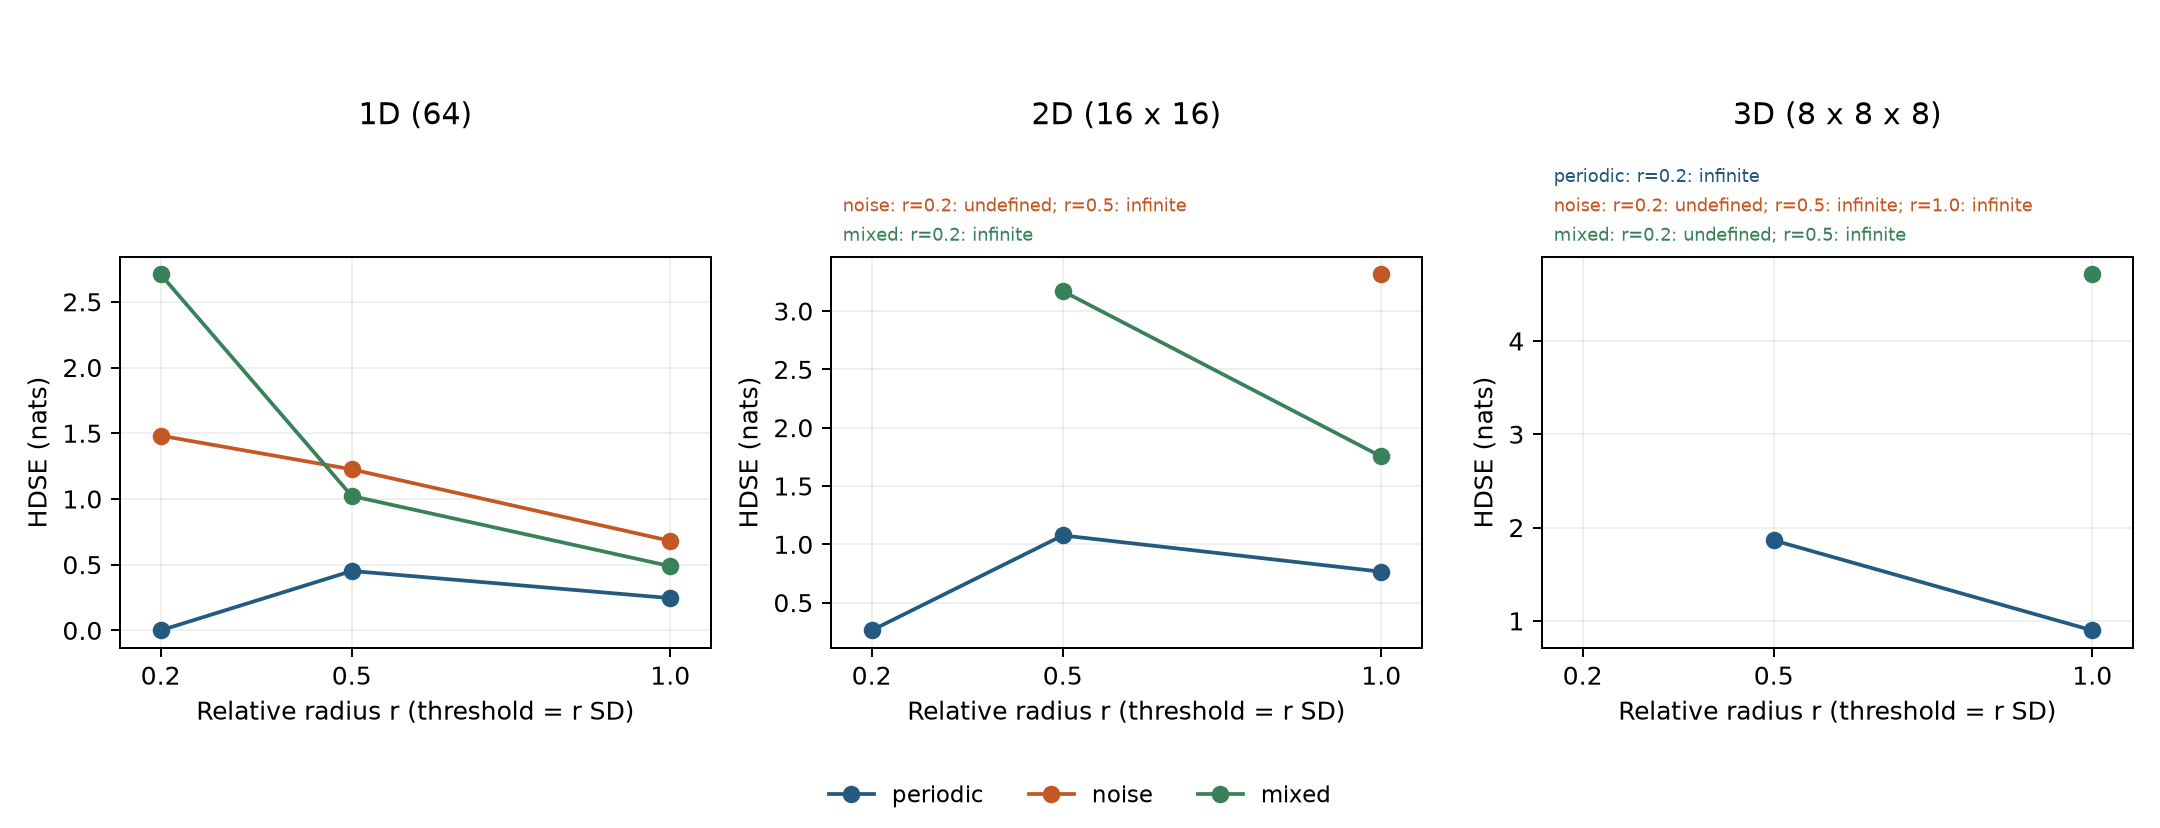
\includegraphics[width=1\linewidth,height=0.9\textheight,keepaspectratio,alt={Baseline HDSE tolerance demonstration. Finite estimates are plotted; undefined and infinite estimates remain annotated and recorded in the table.}]{../figures/hdse-tolerance.png}
\caption{Baseline HDSE tolerance demonstration. Finite estimates are
plotted; undefined and infinite estimates remain annotated and recorded
in the table.}\label{fig:baseline}
\end{figure}

\subsection{Replicated native HDSE}\label{replicated-native-hdse}

The replicated report contains 150 fields and 1650 estimates: 1528
finite, 105 undefined and 17 infinite. The tables retain the finite
conditional mean and sample SD, the finite fraction and the
undefined/infinite counts (U/I). A dash indicates an unavailable finite
mean or SD; it does not denote zero entropy.

{\def\LTcaptype{none} % do not increment counter
\begin{longtable}[]{@{}lllllll@{}}
\toprule\noalign{}
Shape & \(p\) & \(r\) & Mean & SD & Finite/n & U/I \\
\midrule\noalign{}
\endhead
\bottomrule\noalign{}
\endlastfoot
6x7x8 & 0 & 1.5 & 0.620344 & 0 & 5/5 & 0/0 \\
6x7x8 & 0 & 2 & 0.334022 & 0 & 5/5 & 0/0 \\
6x7x8 & 0 & 2.5 & 0.181913 & 0 & 5/5 & 0/0 \\
6x7x8 & 0.25 & 1.5 & 3.71297 & 1.44226 & 5/5 & 0/0 \\
6x7x8 & 0.25 & 2 & 2.21524 & 0.731486 & 5/5 & 0/0 \\
6x7x8 & 0.25 & 2.5 & 1.18716 & 0.254853 & 5/5 & 0/0 \\
6x7x8 & 0.5 & 1.5 & 5.22817 & 0.343375 & 3/5 & 0/2 \\
6x7x8 & 0.5 & 2 & 2.40793 & 0.402156 & 5/5 & 0/0 \\
6x7x8 & 0.5 & 2.5 & 1.14763 & 0.136496 & 5/5 & 0/0 \\
6x7x8 & 0.75 & 1.5 & 5.2898 & 0.184894 & 2/5 & 0/3 \\
6x7x8 & 0.75 & 2 & 3.29457 & 0.316691 & 5/5 & 0/0 \\
6x7x8 & 0.75 & 2.5 & 1.44975 & 0.191395 & 5/5 & 0/0 \\
6x7x8 & 1 & 1.5 & - & - & 0/5 & 0/5 \\
6x7x8 & 1 & 2 & 4.14886 & 0.305753 & 5/5 & 0/0 \\
6x7x8 & 1 & 2.5 & 1.68958 & 0.112868 & 5/5 & 0/0 \\
10x12 & 0 & 1.5 & 0.195222 & 0 & 5/5 & 0/0 \\
10x12 & 0 & 2 & 0.0950618 & 0 & 5/5 & 0/0 \\
10x12 & 0 & 2.5 & 0.0471768 & 0 & 5/5 & 0/0 \\
10x12 & 0.25 & 1.5 & 0.845984 & 0.198192 & 5/5 & 0/0 \\
10x12 & 0.25 & 2 & 0.412154 & 0.0775165 & 5/5 & 0/0 \\
10x12 & 0.25 & 2.5 & 0.204453 & 0.0403457 & 5/5 & 0/0 \\
10x12 & 0.5 & 1.5 & 1.39016 & 0.187022 & 5/5 & 0/0 \\
10x12 & 0.5 & 2 & 0.637592 & 0.0698127 & 5/5 & 0/0 \\
10x12 & 0.5 & 2.5 & 0.301306 & 0.0347635 & 5/5 & 0/0 \\
10x12 & 0.75 & 1.5 & 1.84024 & 0.161139 & 5/5 & 0/0 \\
10x12 & 0.75 & 2 & 0.977935 & 0.0408192 & 5/5 & 0/0 \\
10x12 & 0.75 & 2.5 & 0.434886 & 0.0426958 & 5/5 & 0/0 \\
10x12 & 1 & 1.5 & 2.00003 & 0.179567 & 5/5 & 0/0 \\
10x12 & 1 & 2 & 1.06436 & 0.127857 & 5/5 & 0/0 \\
10x12 & 1 & 2.5 & 0.425303 & 0.0656491 & 5/5 & 0/0 \\
48 & 0 & 1.5 & 0.163193 & 0 & 5/5 & 0/0 \\
48 & 0 & 2 & 0.0943835 & 0 & 5/5 & 0/0 \\
48 & 0 & 2.5 & 0.0497278 & 0 & 5/5 & 0/0 \\
48 & 0.25 & 1.5 & 0.34872 & 0.0451071 & 5/5 & 0/0 \\
48 & 0.25 & 2 & 0.190946 & 0.0265122 & 5/5 & 0/0 \\
48 & 0.25 & 2.5 & 0.0761487 & 0.0129646 & 5/5 & 0/0 \\
48 & 0.5 & 1.5 & 0.395644 & 0.0426951 & 5/5 & 0/0 \\
48 & 0.5 & 2 & 0.189375 & 0.0111342 & 5/5 & 0/0 \\
48 & 0.5 & 2.5 & 0.0752926 & 0.00613628 & 5/5 & 0/0 \\
48 & 0.75 & 1.5 & 0.387622 & 0.0279628 & 5/5 & 0/0 \\
48 & 0.75 & 2 & 0.196965 & 0.023594 & 5/5 & 0/0 \\
48 & 0.75 & 2.5 & 0.0802966 & 0.00841765 & 5/5 & 0/0 \\
48 & 1 & 1.5 & 0.415829 & 0.022104 & 5/5 & 0/0 \\
48 & 1 & 2 & 0.237607 & 0.0212663 & 5/5 & 0/0 \\
48 & 1 & 2.5 & 0.0810962 & 0.015752 & 5/5 & 0/0 \\
\end{longtable}
}

\begin{figure}
\centering
\includegraphics[width=1\linewidth,height=0.9\textheight,keepaspectratio,alt={Native HDSE across Bernoulli replacement probabilities and configured radii. Finite conditional summaries are accompanied by outcome counts; variability is across generated fields, not template pairs.}]{../figures/mix-entropy.png}
\caption{Native HDSE across Bernoulli replacement probabilities and
configured radii. Finite conditional summaries are accompanied by
outcome counts; variability is across generated fields, not template
pairs.}\label{fig:mix}
\end{figure}

\begin{figure}
\centering
\includegraphics[width=1\linewidth,height=0.9\textheight,keepaspectratio,alt={Finite, undefined and infinite outcomes across the replicated design. These statuses are retained rather than imputed as zero.}]{../figures/degeneracy.png}
\caption{Finite, undefined and infinite outcomes across the replicated
design. These statuses are retained rather than imputed as
zero.}\label{fig:degeneracy}
\end{figure}

Matching probabilities provide another view of these outcomes. A
positive base count followed by zero extended matches gives infinite
continuation entropy; zero base matches give undefined entropy.
Increasing native feature count and changing spatial geometry can
therefore affect interpretability even when all input amplitudes are
valid.

\begin{figure}
\centering
\includegraphics[width=1\linewidth,height=0.9\textheight,keepaspectratio,alt={Base and extended template matching probabilities from observed pair counts. Sparse extended matches explain finite-sample degeneracy without reinterpreting it as zero entropy.}]{../figures/match-probability.png}
\caption{Base and extended template matching probabilities from observed
pair counts. Sparse extended matches explain finite-sample degeneracy
without reinterpreting it as zero entropy.}\label{fig:matches}
\end{figure}

\subsection{Structured controls and alternative
representations}\label{structured-controls-and-alternative-representations}

{\def\LTcaptype{none} % do not increment counter
\begin{longtable}[]{@{}lllllll@{}}
\toprule\noalign{}
Shape & Control & \(r\) & Mean & SD & Finite/n & U/I \\
\midrule\noalign{}
\endhead
\bottomrule\noalign{}
\endlastfoot
6x7x8 & checkerboard & 1.5 & 0 & 0 & 5/5 & 0/0 \\
6x7x8 & checkerboard & 2 & 0 & 0 & 5/5 & 0/0 \\
6x7x8 & checkerboard & 2.5 & 0 & 0 & 5/5 & 0/0 \\
6x7x8 & constant & 1.5 & - & - & 0/5 & 5/0 \\
6x7x8 & constant & 2 & - & - & 0/5 & 5/0 \\
6x7x8 & constant & 2.5 & - & - & 0/5 & 5/0 \\
6x7x8 & correlated & 1.5 & 2.56749 & 0.840728 & 5/5 & 0/0 \\
6x7x8 & correlated & 2 & 1.37786 & 0.385547 & 5/5 & 0/0 \\
6x7x8 & correlated & 2.5 & 0.753716 & 0.232607 & 5/5 & 0/0 \\
6x7x8 & gaussian & 1.5 & 5.65724 & 0.495324 & 3/5 & 0/2 \\
6x7x8 & gaussian & 2 & 3.3292 & 0.351848 & 5/5 & 0/0 \\
6x7x8 & gaussian & 2.5 & 1.56662 & 0.232115 & 5/5 & 0/0 \\
6x7x8 & shuffled & 1.5 & - & - & 0/5 & 0/5 \\
6x7x8 & shuffled & 2 & 3.35688 & 0.471817 & 5/5 & 0/0 \\
6x7x8 & shuffled & 2.5 & 1.76955 & 0.302802 & 5/5 & 0/0 \\
10x12 & checkerboard & 1.5 & 0 & 0 & 5/5 & 0/0 \\
10x12 & checkerboard & 2 & 0 & 0 & 5/5 & 0/0 \\
10x12 & checkerboard & 2.5 & 0 & 0 & 5/5 & 0/0 \\
10x12 & constant & 1.5 & - & - & 0/5 & 5/0 \\
10x12 & constant & 2 & - & - & 0/5 & 5/0 \\
10x12 & constant & 2.5 & - & - & 0/5 & 5/0 \\
10x12 & correlated & 1.5 & 0.662661 & 0.109864 & 5/5 & 0/0 \\
10x12 & correlated & 2 & 0.367965 & 0.0601135 & 5/5 & 0/0 \\
10x12 & correlated & 2.5 & 0.185265 & 0.0324345 & 5/5 & 0/0 \\
10x12 & gaussian & 1.5 & 1.74544 & 0.233531 & 5/5 & 0/0 \\
10x12 & gaussian & 2 & 0.861448 & 0.128388 & 5/5 & 0/0 \\
10x12 & gaussian & 2.5 & 0.400276 & 0.0465602 & 5/5 & 0/0 \\
10x12 & shuffled & 1.5 & 1.79204 & 0.0637443 & 5/5 & 0/0 \\
10x12 & shuffled & 2 & 0.850403 & 0.0587828 & 5/5 & 0/0 \\
10x12 & shuffled & 2.5 & 0.409024 & 0.027914 & 5/5 & 0/0 \\
48 & checkerboard & 1.5 & 0 & 0 & 5/5 & 0/0 \\
48 & checkerboard & 2 & 0 & 0 & 5/5 & 0/0 \\
48 & checkerboard & 2.5 & 0 & 0 & 5/5 & 0/0 \\
48 & constant & 1.5 & - & - & 0/5 & 5/0 \\
48 & constant & 2 & - & - & 0/5 & 5/0 \\
48 & constant & 2.5 & - & - & 0/5 & 5/0 \\
48 & correlated & 1.5 & 0.139492 & 0.0537352 & 5/5 & 0/0 \\
48 & correlated & 2 & 0.0738259 & 0.0204956 & 5/5 & 0/0 \\
48 & correlated & 2.5 & 0.0390499 & 0.0114501 & 5/5 & 0/0 \\
48 & gaussian & 1.5 & 0.354011 & 0.0389952 & 5/5 & 0/0 \\
48 & gaussian & 2 & 0.172839 & 0.026053 & 5/5 & 0/0 \\
48 & gaussian & 2.5 & 0.0831918 & 0.0118893 & 5/5 & 0/0 \\
48 & shuffled & 1.5 & 0.360859 & 0.0357175 & 5/5 & 0/0 \\
48 & shuffled & 2 & 0.208973 & 0.018994 & 5/5 & 0/0 \\
48 & shuffled & 2.5 & 0.0736555 & 0.00547319 & 5/5 & 0/0 \\
\end{longtable}
}

\begin{figure}
\centering
\includegraphics[width=1\linewidth,height=0.9\textheight,keepaspectratio,alt={Native spatial HDSE and row-major flattened sample entropy. Their template feature counts and extension geometries differ; the comparison does not isolate flattening alone.}]{../figures/native-v-flattened.png}
\caption{Native spatial HDSE and row-major flattened sample entropy.
Their template feature counts and extension geometries differ; the
comparison does not isolate flattening alone.}\label{fig:geometry}
\end{figure}

The geometry comparison is read together with feature counts and
populations. Neither a difference nor an agreement alone establishes
estimator superiority. The observed tables are specific to the declared
synthetic design, radius, finite sample and block geometry.

\subsection{Related entropy and statistical
complexity}\label{related-entropy-and-statistical-complexity}

The recorded normalization options make these related-measure summaries
dimensionless. Display labels are DistEn: distribution entropy; PermEn:
permutation; Spectral: spectral; Shannon: shannon; C-JS: statistical
complexity.

{\def\LTcaptype{none} % do not increment counter
\begin{longtable}[]{@{}lllllll@{}}
\toprule\noalign{}
Shape & \(p\) & Estimator & Finite mean & SD & Finite/n & U/I \\
\midrule\noalign{}
\endhead
\bottomrule\noalign{}
\endlastfoot
6x7x8 & 0 & DistEn & 0.821272 & 0 & 5/5 & 0/0 \\
6x7x8 & 0 & PermEn & 0.401562 & 0 & 5/5 & 0/0 \\
6x7x8 & 0 & Spectral & 0.366254 & 0 & 5/5 & 0/0 \\
6x7x8 & 0 & Shannon & 0.655986 & 0 & 5/5 & 0/0 \\
6x7x8 & 0 & C-JS & 0.304078 & 0 & 5/5 & 0/0 \\
6x7x8 & 0.25 & DistEn & 0.895451 & 0.00818597 & 5/5 & 0/0 \\
6x7x8 & 0.25 & PermEn & 0.496046 & 0.00286137 & 5/5 & 0/0 \\
6x7x8 & 0.25 & Spectral & 0.817511 & 0.0262881 & 5/5 & 0/0 \\
6x7x8 & 0.25 & Shannon & 0.723031 & 0.00469153 & 5/5 & 0/0 \\
6x7x8 & 0.25 & C-JS & 0.278564 & 0.00207836 & 5/5 & 0/0 \\
6x7x8 & 0.5 & DistEn & 0.851999 & 0.00667078 & 5/5 & 0/0 \\
6x7x8 & 0.5 & PermEn & 0.503431 & 0.000895235 & 5/5 & 0/0 \\
6x7x8 & 0.5 & Spectral & 0.908797 & 0.0156529 & 5/5 & 0/0 \\
6x7x8 & 0.5 & Shannon & 0.744093 & 0.00724335 & 5/5 & 0/0 \\
6x7x8 & 0.5 & C-JS & 0.274515 & 0.00490519 & 5/5 & 0/0 \\
6x7x8 & 0.75 & DistEn & 0.829532 & 0.00809795 & 5/5 & 0/0 \\
6x7x8 & 0.75 & PermEn & 0.503852 & 0.000556784 & 5/5 & 0/0 \\
6x7x8 & 0.75 & Spectral & 0.923803 & 0.00685935 & 5/5 & 0/0 \\
6x7x8 & 0.75 & Shannon & 0.727915 & 0.00931895 & 5/5 & 0/0 \\
6x7x8 & 0.75 & C-JS & 0.28245 & 0.00532371 & 5/5 & 0/0 \\
6x7x8 & 1 & DistEn & 0.813712 & 0.00826181 & 5/5 & 0/0 \\
6x7x8 & 1 & PermEn & 0.503478 & 0.000811645 & 5/5 & 0/0 \\
6x7x8 & 1 & Spectral & 0.923819 & 0.00686466 & 5/5 & 0/0 \\
6x7x8 & 1 & Shannon & 0.657322 & 0.00954592 & 5/5 & 0/0 \\
6x7x8 & 1 & C-JS & 0.317542 & 0.00516416 & 5/5 & 0/0 \\
10x12 & 0 & DistEn & 0.9211 & 0 & 5/5 & 0/0 \\
10x12 & 0 & PermEn & 0.630036 & 0 & 5/5 & 0/0 \\
10x12 & 0 & Spectral & 0.322933 & 0 & 5/5 & 0/0 \\
10x12 & 0 & Shannon & 0.702175 & 0 & 5/5 & 0/0 \\
10x12 & 0 & C-JS & 0.288771 & 0 & 5/5 & 0/0 \\
10x12 & 0.25 & DistEn & 0.919696 & 0.0121944 & 5/5 & 0/0 \\
10x12 & 0.25 & PermEn & 0.918879 & 0.0172518 & 5/5 & 0/0 \\
10x12 & 0.25 & Spectral & 0.659491 & 0.0456326 & 5/5 & 0/0 \\
10x12 & 0.25 & Shannon & 0.712075 & 0.00929196 & 5/5 & 0/0 \\
10x12 & 0.25 & C-JS & 0.288816 & 0.00161396 & 5/5 & 0/0 \\
10x12 & 0.5 & DistEn & 0.895524 & 0.0103245 & 5/5 & 0/0 \\
10x12 & 0.5 & PermEn & 0.943309 & 0.0145696 & 5/5 & 0/0 \\
10x12 & 0.5 & Spectral & 0.827952 & 0.0306717 & 5/5 & 0/0 \\
10x12 & 0.5 & Shannon & 0.704415 & 0.00672185 & 5/5 & 0/0 \\
10x12 & 0.5 & C-JS & 0.293462 & 0.00222378 & 5/5 & 0/0 \\
10x12 & 0.75 & DistEn & 0.884852 & 0.00745327 & 5/5 & 0/0 \\
10x12 & 0.75 & PermEn & 0.96377 & 0.00709848 & 5/5 & 0/0 \\
10x12 & 0.75 & Spectral & 0.902698 & 0.0121331 & 5/5 & 0/0 \\
10x12 & 0.75 & Shannon & 0.683502 & 0.0056531 & 5/5 & 0/0 \\
10x12 & 0.75 & C-JS & 0.302502 & 0.00211954 & 5/5 & 0/0 \\
10x12 & 1 & DistEn & 0.895472 & 0.00992491 & 5/5 & 0/0 \\
10x12 & 1 & PermEn & 0.965971 & 0.00735781 & 5/5 & 0/0 \\
10x12 & 1 & Spectral & 0.91021 & 0.0134747 & 5/5 & 0/0 \\
10x12 & 1 & Shannon & 0.66164 & 0.00852925 & 5/5 & 0/0 \\
10x12 & 1 & C-JS & 0.31495 & 0.00483384 & 5/5 & 0/0 \\
48 & 0 & DistEn & 0.909918 & 0 & 5/5 & 0/0 \\
48 & 0 & PermEn & 0.999673 & 0 & 5/5 & 0/0 \\
48 & 0 & Spectral & 0.179052 & 0 & 5/5 & 0/0 \\
48 & 0 & Shannon & 0.5 & 0 & 5/5 & 0/0 \\
48 & 0 & C-JS & 0.331184 & 0 & 5/5 & 0/0 \\
48 & 0.25 & DistEn & 0.915257 & 0.00752288 & 5/5 & 0/0 \\
48 & 0.25 & PermEn & 0.993391 & 0.0035118 & 5/5 & 0/0 \\
48 & 0.25 & Spectral & 0.777561 & 0.0341609 & 5/5 & 0/0 \\
48 & 0.25 & Shannon & 0.578943 & 0.0354646 & 5/5 & 0/0 \\
48 & 0.25 & C-JS & 0.325202 & 0.00666305 & 5/5 & 0/0 \\
48 & 0.5 & DistEn & 0.929259 & 0.00851251 & 5/5 & 0/0 \\
48 & 0.5 & PermEn & 0.986552 & 0.00983542 & 5/5 & 0/0 \\
48 & 0.5 & Spectral & 0.845927 & 0.0531868 & 5/5 & 0/0 \\
48 & 0.5 & Shannon & 0.613281 & 0.0207336 & 5/5 & 0/0 \\
48 & 0.5 & C-JS & 0.322901 & 0.00458086 & 5/5 & 0/0 \\
48 & 0.75 & DistEn & 0.948009 & 0.0133912 & 5/5 & 0/0 \\
48 & 0.75 & PermEn & 0.993387 & 0.00574809 & 5/5 & 0/0 \\
48 & 0.75 & Spectral & 0.882617 & 0.0293371 & 5/5 & 0/0 \\
48 & 0.75 & Shannon & 0.629339 & 0.0270578 & 5/5 & 0/0 \\
48 & 0.75 & C-JS & 0.320595 & 0.00573027 & 5/5 & 0/0 \\
48 & 1 & DistEn & 0.958792 & 0.00697917 & 5/5 & 0/0 \\
48 & 1 & PermEn & 0.999151 & 0.00116918 & 5/5 & 0/0 \\
48 & 1 & Spectral & 0.880134 & 0.0274742 & 5/5 & 0/0 \\
48 & 1 & Shannon & 0.63448 & 0.0272821 & 5/5 & 0/0 \\
48 & 1 & C-JS & 0.318596 & 0.00497193 & 5/5 & 0/0 \\
\end{longtable}
}

\begin{figure}
\centering
\includegraphics[width=1\linewidth,height=0.9\textheight,keepaspectratio,alt={Normalized Shannon entropy and Jensen-Shannon statistical complexity of the complete configured fixed-bin amplitude alphabet. This is a descriptive distributional extension, not a causal ordinal classification.}]{../figures/entropy-complexity.png}
\caption{Normalized Shannon entropy and Jensen-Shannon statistical
complexity of the complete configured fixed-bin amplitude alphabet. This
is a descriptive distributional extension, not a causal ordinal
classification.}\label{fig:statistical}
\end{figure}

The entropy-complexity plane separates distributional uncertainty from
distance to the uniform alphabet. A high normalized entropy and a high
statistical complexity are different conditions. These
fixed-amplitude-bin observations do not carry the causal ordinal
interpretation of a Bandt-Pompe analysis.

\section{Reproducibility and software
architecture}\label{sec:reproducibility}

\subsection{Numerical and file
boundaries}\label{numerical-and-file-boundaries}

The numerical package separates array validation, geometry, blocked pair
work and estimator-specific semantics. It does not import manuscript or
plotting tooling. Immutable configurations reject unknown options. The
registry binds the complete call signature, distinguishes observations
from probability alphabets and retains effective parameters in every
result. NPY loading disables pickle; CSV inputs retain their declared
grid meaning. Strict JSON represents nonfinite estimates through
explicit statuses and null values.

Tests use analytical examples, independently computed loop oracles,
seeded arrays, real files and actual subprocesses. Deliberately invalid
inputs and coherently altered artifact records are controls proving that
checks can fail. Configured coverage floors are 90 percent for numerical
source and 60 percent for research infrastructure.

The configured verification receipts report 613 passing tests, 95.6492
percent source coverage and 88.4959 percent infrastructure coverage.
These are recorded runs, not a substitute for independent release
review.

Receipt identities (SHA-256):

\begingroup\small

\begin{Shaded}
\begin{Highlighting}[]
\NormalTok{Source coverage: 482700cb812cba4b713afe1e47d1cadec4474b26c3ba8a9cc0631ba283e9987f}
\NormalTok{Infra coverage:  c3febbc9fb7a4ef63c2eda9cda2e8704f959960802a1597b5dad59cffcc352a5}
\NormalTok{Test log:        22b78552a93712b0018ed744b6519438fab29689ca6750dfb4a9186ae7cfee4c}
\end{Highlighting}
\end{Shaded}

\endgroup

\subsection{Source-bound manuscript
generation}\label{source-bound-manuscript-generation}

The title, author metadata, version, design, measurements, tables and
figure paths are sourced from the validated publication profile, project
manifest and generated reports. Template variables must all resolve
before rendering. The shared implementation is
\href{https://github.com/docxology/template}{docxology/template}, pinned
at \breaktt{d39f2478da2512b42ad961e98a5f3b854723f92e}, using the
canonical \breaktt{projects/templates/template\_code\_project/manuscript}
conventions. Actual installed Python and Lua source files are
authenticated against their installer RECORD hashes. Pandoc,
Pandoc-crossref, BibTeX and the selected LaTeX engine produce
mathematical typesetting, resolved references and a real TOC. No custom
ReportLab manuscript fallback is used.

The inspectable resolved section tree, variable inventory, renderer
source/tool receipt, generated TeX/TOC diagnostics and final PDF remain
distinct artifacts. Figure staging uses exact-byte copies of producer
outputs because the shared PDF renderer expects a sibling figure
directory. Staging does not recompute or alter those figures.

\subsection{Provenance bindings}\label{provenance-bindings}

\begingroup\small

\begin{Shaded}
\begin{Highlighting}[]
\NormalTok{Results CSV SHA{-}256: a4104429035874774f07cb2ec816a1cd656504435f245754d730e3bc06526727}
\NormalTok{Study CSV SHA{-}256: 493fd105d2410a1ac66c3bcf75e2a0313dc69e7b6ccd58625508454cc3ae57ce}
\NormalTok{Study report SHA{-}256: e77af9a7e5a55ddca73d9f779e55cf5e715d60e77b0fadd7c93f91f409f425be}
\end{Highlighting}
\end{Shaded}

\endgroup

The manifest binds actual input, configuration, code and output bytes.
Stored file, canonical array, configuration, result and table identities
remain exact. Synthetic design replay alone uses a declared,
machine-epsilon-derived float64 envelope after exact shape and
finite-value checks. This accommodates bounded platform roundoff without
changing stored inputs, smoothing matching thresholds or relabeling
stale results. The initial hosted failure and its adversarial regression
controls are retained in the project record.

The supplied published PDF is not redistributed. No project DOI, journal
acceptance, empirical source-paper replication or independent
application validation is claimed by the software build. Independent
scientific and release review remains separate from these executable
engineering checks.

\section{Discussion and conclusions}\label{sec:conclusion}

Native geometry, input meaning and estimator convention are parts of a
complexity analysis rather than preprocessing details that can be
silently discarded. The framework makes those choices configurable and
records their numerical consequences with counts and explicit statuses.
The replicated study and computational records allow readers to examine
tolerance, spatial representation, degeneracy and resource use together.

Finite conditional summaries must be interpreted alongside all outcome
counts. The high-dimensional template feature population and finite
origin geometry change together, while the native-versus-flattened
comparison also changes continuation length. Stable ordinal ties,
amplitude binning, spectral preprocessing and singular-value
normalization are documented conventions. They remain application
choices rather than universal definitions of complexity.

Exhaustive matching is quadratic in templates. Blocking bounds
workspace, and the analytical estimator exposes the work schedule, but
neither removes that growth. Host benchmarks describe observed execution
on fixed inputs. New applications may require different data sizes,
symbolization, boundary treatment or more efficient exact and
approximate search methods, each with a new validation contract.

Ant collective behavior and other spatial scientific applications are
future empirical domains, not findings of this synthetic study. Progress
in those domains requires controlled measurements, appropriate null
models, sensitivity analysis and independent review. The present
contribution is a reproducible, typed methods implementation and
source-bound research workflow through which those questions can be
investigated.

\section*{References}\label{references}
\addcontentsline{toc}{section}{References}

Method definitions are attributed to their primary sources. The HDSE
source, the local-template families, probability information,
ordinal/decomposition methods and statistical-complexity family have
separate citation records. Bibliographic entries are resolved by the
shared template's native bibliography pipeline; source metadata do not
import the template exemplar's publication DOI.



\providecommand{\bibsection}{}
\renewcommand{\bibsection}{}

\bibliography{references}
\end{document}
